\documentclass{beamer}
\usepackage{bookmark}
\usepackage{beamerthemeBerkeley}
\usepackage{color}
\usepackage{amsmath}
\usepackage{hyperref}
\hypersetup{colorlinks,linkcolor=blue,citecolor=blue}
\usepackage{listings}
\usepackage{xcolor}
\usepackage{graphicx}
\usepackage{amsfonts}
\usecolortheme{default}
\lstset{
numbers=left,
showspaces=false,
showstringspaces=false,
xleftmargin=.05\textwidth,
frame=shadowbox,
commentstyle=\color{red!80!green!80!blue!80},
}
\title{Fast/Discrete Fourier Transform}
\author{Group 23}
\institute{UM-SJTU Joint Institute}
\date{\today}

\begin{document}
\begin{frame}
	\titlepage
\end{frame}

\begin{frame}
	\tableofcontents
\end{frame}


\begin{frame}
	\section{Introduction}
	\frametitle{Fourier Transform}
	\begin{block}{Definition}
		Fourier transform is a decomposition of a funtion of time (a signal) into frequencies that make it up.
    \end{block}
    \begin{itemize}
        \item The main strategy is to see signals as acuumulations of sine waves of different frequencies, and this can be represented as the following $$f(x) = \int_{-\infty}^{\infty}F(s)e^{2i\pi sx} ds$$
    \end{itemize}
\end{frame}

\begin{frame}
	\frametitle{Discrete Fourier Transform}
    \begin{block}{Limitation on FT}
        In fourier transform, both data in the time domain and frequency domain are {\color{blue} continuous}, which are not feasible to store and process in computers.
    \end{block}

	\vskip 2em
	Discrete Fourier Transform (DFT) solves this question as it processes a {\color{blue} finite sample sequence} of time domain data and convert it into a same-length sample data for frequency domain.
\end{frame}

\begin{frame}
	\frametitle{Mathematical Formula}
    DFT will decompose a sequence $\{x_n\}$ of length $N$ into the following style $$x_n = \frac{1}{N}\sum_{k=0}^{N-1}X_k\cdot e^{i2\pi kn/N}$$

    And thus the sequence $X_k$ which represents how much a certain frequency is in the sample can be written as $$X_k = \sum_{n=0}^{N-1}x_n\cdot e^{i2\pi kn/N}$$
\end{frame}

\begin{frame}
	\section{Fast Fourier Transform}
	\frametitle{Fast Fourier Transform}
    If the calculation of $DFT$ is operated naively, then it is clear that the time complexity is $\mathcal{O}(n^2)$ for a length-$n$ sequence.

    \vskip 2em
    
    And thus Fast Fourier Transform(FFT) is introduced, which serves to find the internal mathematical basis and simplify the calculation, usually to $\mathcal{O}(n\log{n})$. And here the algorithm introduced will be {\color{blue} Cooley-Tukey algorithm}

    The algorithm uses the idea of divide and conquer, so here the case when $n=2^{p}$ is considered.
\end{frame}

\begin{frame}
	\subsection{Cooley-Tukey Algorithm}
    \frametitle{Cooley-Tukey Algorithm}
    $a$: input sequence, $A$: output sequence

    $W$: $e^{-i2\pi /n }$, $weight_{j,k} = W^{\frac{8}{2^j}\times k}$
    
    \begin{figure}
        \centering
        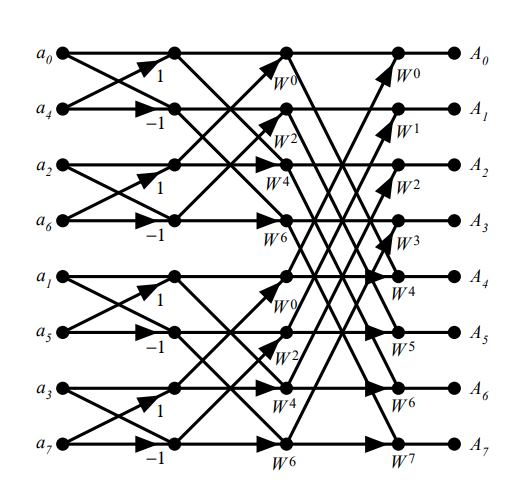
\includegraphics[scale=0.5]{../problem38_1.png}
    \end{figure}
	
\end{frame}


\begin{frame}
	\section{References}
	\frametitle{References}
	\begin{itemize}\itemsep .125cm
        \item \url{https://www.cs.cmu.edu/afs/andrew/scs/cs/15-463/2001/pub/www/notes/fourier/fourier.pdf}
        \item James W. Cooley, Peter A. W. Lewis, and Peter W. Welch, "Historical notes on the fast Fourier transform"
        \item \url{https://en.wikipedia.org/wiki/Fast_Fourier_transform}
    \end{itemize}
\end{frame}

\end{document}